\documentclass[a4paper,article,14pt]{extarticle}

\usepackage{spbudiploma}
\usepackage{amsmath}
\usepackage{mathtools}
\usepackage[pdftex]{graphicx}
\graphicspath{{../pictures/}}
\usepackage{listings}
\usepackage{xcolor}
\usepackage{amsfonts}
\usepackage{amsmath}
\usepackage{cases}

\usepackage{enumitem}
\definecolor{codegreen}{rgb}{0,0.6,0}
\definecolor{codegray}{rgb}{0.5,0.5,0.5}
\definecolor{codepurple}{rgb}{0.58,0,0.82}
\definecolor{backcolour}{rgb}{0.95,0.95,0.92}

\lstdefinestyle{mystyle}{
	backgroundcolor=\color{backcolour},   
	commentstyle=\color{codegreen},
	keywordstyle=\color{codegreen},
	numberstyle=\tiny\color{codegray},
	stringstyle=\color{codepurple},
	basicstyle=\ttfamily\footnotesize,
	breakatwhitespace=false,         
	breaklines=true,                 
	captionpos=b,                    
	keepspaces=false,                 
	numbers=left,                    
	numbersep=5pt,                  
	showspaces=false,                
	showstringspaces=false,
	showtabs=false,                  
	tabsize=2
}

\lstset{style=mystyle}

\begin{document}
	\begin{titlepage}
		\begin{center}
			FEDERAL STATE AUTONOMOUS EDUCATIONAL INSTITUTION
			
			OF HIGHER EDUCATION
			
			ITMO UNIVERSITY
			\vspace{3cm}
			
			\large\textbf{Report}
			
			\large on the practical task No. 4
			
			\large \flqq Algorithms for unconstrained nonlinear optimization. \\ Stochastic and metaheuristic algorithms\frqq
			\vspace{5cm}
			

			\begin{flushright}
				{Performed by:} \\
				Putnikov Semyon \\ 
				J4132c \\
			\end{flushright}
			
			
			\begin{flushright}
				{Accepted by:} \\
				Dr Petr Chunaev \\ 
			\end{flushright}
			\vfill
			
			{St. Petersburg}
			\par{\number\year}
		\end{center}
	\end{titlepage}

	\newpage
	
	\section{Goal}
	The use of stochastic and metaheuristic algorithms (Simulated Annealing, Differential Evolution, Particle Swarm Optimization) in the tasks of unconstrained nonlinear optimization and the experimental comparison of them with Nelder-Mead and Levenberg-Marquardt algorithms.
	
	\section{Formulation of the problem}
	Generate the noisy data $(x_k,y_k)$, where $k=0,…,1000$, according to the rule:
	\begin{numcases}{f(x)=}
		-100+\delta_k, & \text{$f(x_k) < -100$}\\
		f(x_k)+\delta_k, & \text{$-100 \leq f(x_k) \leq 100, x_k = \frac{3k}{1000}$}\\
		100 + \delta_k, & \text{$f(x_k)>100$}
	\end{numcases}
	
	$$f(x)=\frac{1}{(x^2-3x+2)}$$
	
	where $\delta_k\sim\textit{N}(0,1)$ are values of a random variable with standard normal distribution. Approximate the data by the rational function $$F(x,a,b,c,d)=\frac{ax+b}{^2+cx+d}$$ by means of least squares through the numerical minimization of the following function: $$D(a,b,c,d) = \sum\limits_{k=0}^{1000} (F(x_k,a,b,c,d)-y_k)^2$$
	
	To solve the minimization problem, use Nelder-Mead algorithm, Levenberg-Marquardt algorithm and at least two of the methods among Simulated Annealing, Differential Evolution and Particle Swarm Optimization. If necessary, set the initial approximations and other parameters of the methods. Use $\epsilon=0.001$ as the precision; at most 1000 iterations are allowed. Visualize the data and the approximants obtained in a single plot. Analyze and compare the results obtained (in terms of number of iterations, precision, number of function evaluations, etc.).
	
	\section{Brief theoretical part}
	\subsection{Nelder-Mead algorithm}
	The Nelder–Mead method is a commonly applied numerical method used to find the minimum or maximum of an objective function in a multidimensional space. The method uses the concept of a simplex, which is a special polytope of n + 1 vertices in n dimensions. Examples of simplices include a line segment on a line, a triangle on a plane, a tetrahedron in three-dimensional space and so forth. 
	
	The method approximates a local optimum of a problem with $n$ variables when the objective function varies smoothly and is unimodal. Typical implementations minimize functions, and we maximize $f(x)$ by minimizing $-f(x)$. Nelder–Mead in n dimensions maintains a set of $n + 1$ test points arranged as a simplex. It then extrapolates the behavior of the objective function measured at each test point in order to find a new test point and to replace one of the old test points with the new one, and so the technique progresses. 
	
	The simplest approach is to replace the worst point with a point reflected through the centroid of the remaining n points. If this point is better than the best current point, then we can try stretching exponentially out along this line. On the other hand, if this new point isn't much better than the previous value, then we are stepping across a valley, so we shrink the simplex towards a better point.
	
	\subsection{Differential Evolution method}
	Differential evolution is an metaheuristic algorithm that solves the optimization problem by maintaining a population of agents, i.e. candidate solutions, creating new agents by combining existing ones and further keeping the best one.
	
	Choose $CR \in [0,1]$, the crossover probability, $F \in[0,2]$, the differential weight, and $NP \geq 4$, the population size. Let $x\in \mathbb{R}^n$ denote an agent in the population.
	
	\subsubsection*{Algorithm}
	Until a termination criterion is met (e.g. the number of iterations performed):
	\begin{itemize}
		\item Randomly pick NP agents \textbf{x} (i.e. the population).
		\item Pick three distinct agents \textbf{a}, \textbf{b} and \textbf{c} from the population, different from \textbf{x}.
		\item Compute the trial vector $y=(y_1,...,y_n)$ as follows. For $i=1,...,n$, pick $r_i\in \mathbb{U}(0,1)$. If $r_i < CR$, then $y_i=a_i + F(b_i - c_i)$, otherwise $y_i = x_i$.
		\item If $f(y)\leq f(x)$, then replace \textbf{x} with the trial vector \textbf{y}, otherwise keep \textbf{x}.
	\end{itemize}
	Pick the best agent from the population and return it as the best found solution.
	
	
	\subsection{Levenberg-Marquardt algorithm}
	The application of LMA is the \textbf{least-squares curve fitting problem}: given a set $(x_i, y_i)_{i=1}^m$, find the parameters $\beta$ (column vector) of the model curve $f(x,\beta)$ so that the sum of the squares of the deviations $S(\beta)$ is minimized: $$arg\min_{\beta} S(\beta)\equiv arg\min_{\beta} \sum_{i=1}^{m}[y_i - f(x_i,\beta)]^2$$
	
	Start with an initial guess for $\beta$. In each iteration step, the parameter vector $\beta$ is replaced by a new estimate $\beta + \Delta \beta$. To determine $\Delta \beta$, the function $f(x_i,\beta + \Delta \beta)$ is approximated by its linearization: $$f(x_i, \beta + \Delta \beta) \approx f(x_i, \beta) + J_i \Delta\beta, J_i = (\nabla_{x_i}f(\beta))^T$$
	
	The sum $S(\beta)$ has its minimum at a zero gradient with respect to $\beta$. The above first-order approximation of $f(x_i, \beta + \Delta \beta)$ gives $$S(\beta + \Delta \beta) \approx \sum_{i=1}^{m} [y_i - f(x_i, \beta) - J_i\Delta \beta]^2$$ or in vector notation, $$S(\beta+ \Delta \beta)\approx[y - f(\beta)]^T [y-f(\beta)]-2[y-f(\beta)]^T J\Delta \beta + \Delta \beta^T J^T J \Delta \beta,$$ where $J$ is the Jacobian matrix, whose i-th row equals $J_i$ , and where $f(\beta)$ and $y$ are vectors with i-th component $f(x_i, \beta)$ and $y_i$ , respectively.
	
	Taking the derivative of $S (\beta + \Delta \beta)$ with respect to $\Delta \beta$ and setting to zero gives $$(J^T J) \Delta \beta = J^T [y - f(\beta)],$$ that is in fact a system of linear equations with respect to $\Delta \beta$.
	
	The system may be replaced by $$(J^T J + \lambda I) \Delta \beta = J^T [y-f(\beta)],$$ where \textbf{I} is the identity matrix, giving the increment $\Delta \beta$ to the estimated parameter vector $\beta$.
	
	\subsection{Particle Swarm Optimization method}
	Particle swarm optimization is a metaheuristic algorithm that solves the optimization problem by iterative moving candidate solutions (particles) with certain velocity. Each particle’s movement is influenced by its local best known position and is guided to the best known positions, which are updated as better positions arefound by other particles.
	
	Let $s$ be the number of particles in the swarm, with positions $x_i$ and velocities $v_i$ . Let $p_i$ be the best known position of particle $i$ and $g$ the one of the entire swarm.
	
	The values $b_l$ and $b_u$ represents the lower and upper boundaries of the search-space. The parameters $\omega$, $\phi_p$, and $\phi_g$ are selected manually and control the behaviour and efficiency of the method.
	
	The choice of parameters can have a large impact on optimization performance and is the subject of much research. Typically, one chooses the parameters for a particular problem with many experiments.
	
	\section{Results}
	%Present the results of solving the assigned problems, including graphs and tables, as well as a brief discussion of the results obtained (at most 4 pages)
	
	All results of calcutions we can see at Figures \ref{results}.
	\begin{figure}[h!]
		\centering
		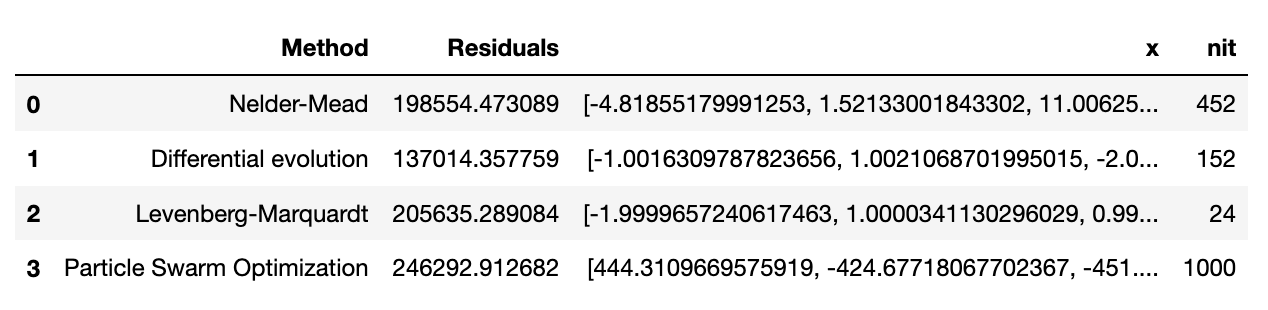
\includegraphics[scale=0.7]{results.png}
		\caption{Results of calcutions.}
		\label{results}
	\end{figure}
	
	\begin{figure}[h!]
		\centering
		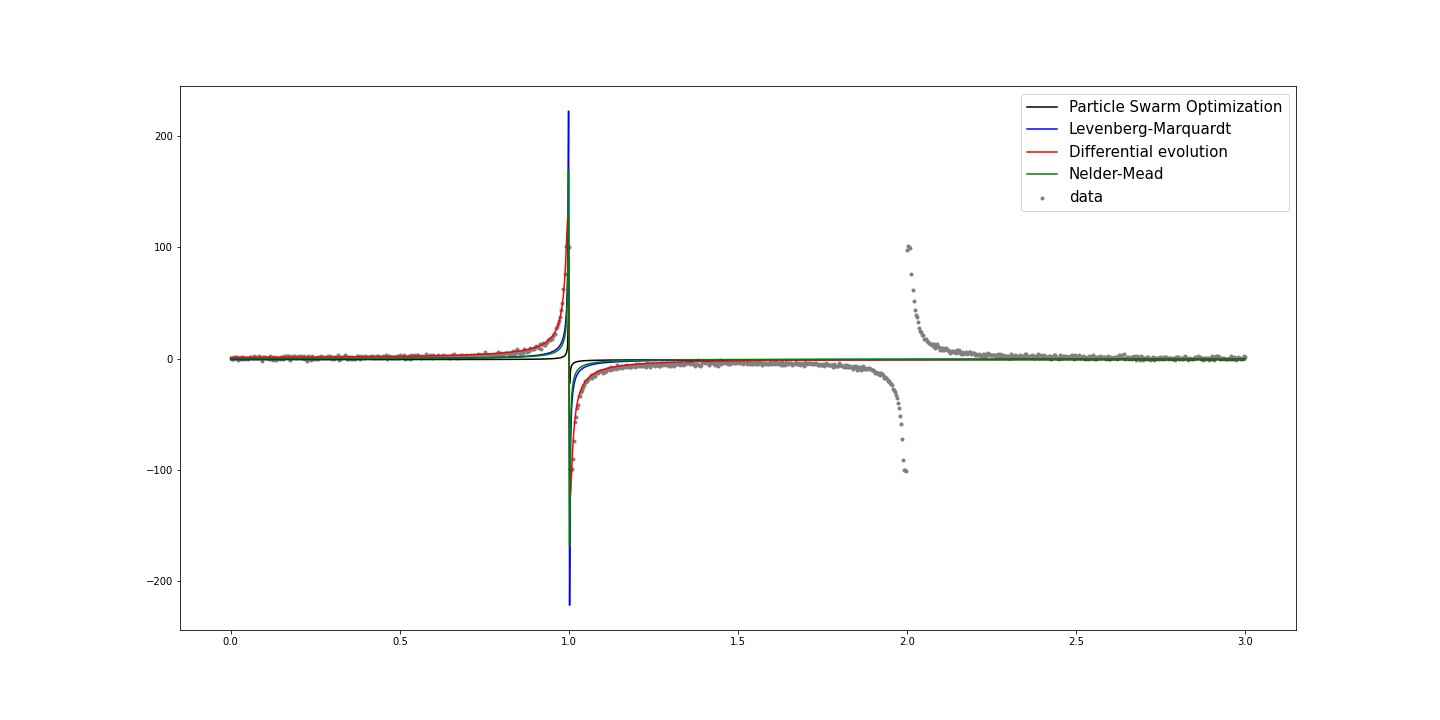
\includegraphics[scale=0.35]{plot_approximation.png}
		\caption{Nelder-Mead algorithm, Differential Evolution method, Levenberg-Marquardt algorithm and Particle Swarm Optimization method.}
		\label{linear}
	\end{figure} 
	
	\begin{figure}[h]
		\centering
		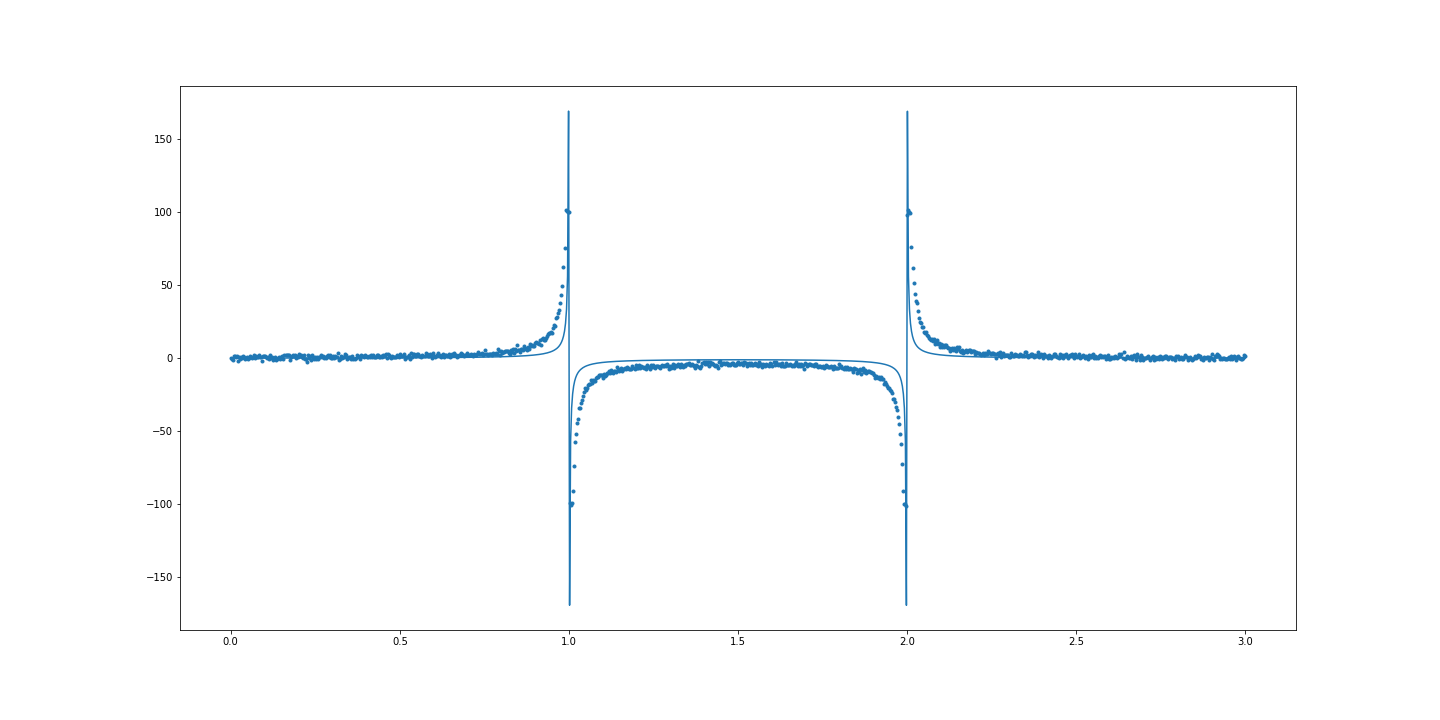
\includegraphics[scale=0.35]{plot_near_min.png}
		\caption{Plot with point near global minimum.}
		\label{rational}
	\end{figure} 
	
	The initial for approximation is complex and non-differentiable. 
	
	The approximation function can’t repeat the behavior of the original function using all of that methods. Nelder-Mead and Levenberg-Marquardt algorithm can’t converce to global minimum without very accurate initial point. They are very sensitive to init point in that case.
	
	Differential evolution show slightly better result and converges with small amount of iterations. To improve result need to make bounds harder and select hyperparameters such as popsize and mutation.
	

	
\end{document}